\section{Hauptteil}
\label{sec:hauptteil}

\subsection{Lesbare Internetadressen}

\subsubsection{Angabe der Unternehmenswebsite}

Die zunächst einfachste Verbindung von Gedrucktem oder vom Schaufenster zu Internetseiten bzw. zum Webshop besteht darin, dem Kunden eine \ac{URL}, also eine Internetadresse\footnote{Obwohl der Begriff URL eine Internetadresse in sehr allgemeiner Form beschreibt, wird er in dieser Arbeit der Lesbarkeit halber synonym zu „WWW--Adresse“ verwendet.} zu nennen, die dieser dann am PC oder per Mobiltelefon aufruft.
Soll lediglich auf die Startseite des Webangebots hingewiesen werden, ist hierzu die gewöhnliche Adresse hier also \url{www.Manufactum.de}, anzugeben. 

\begin{figure}[H]
\begin{center}
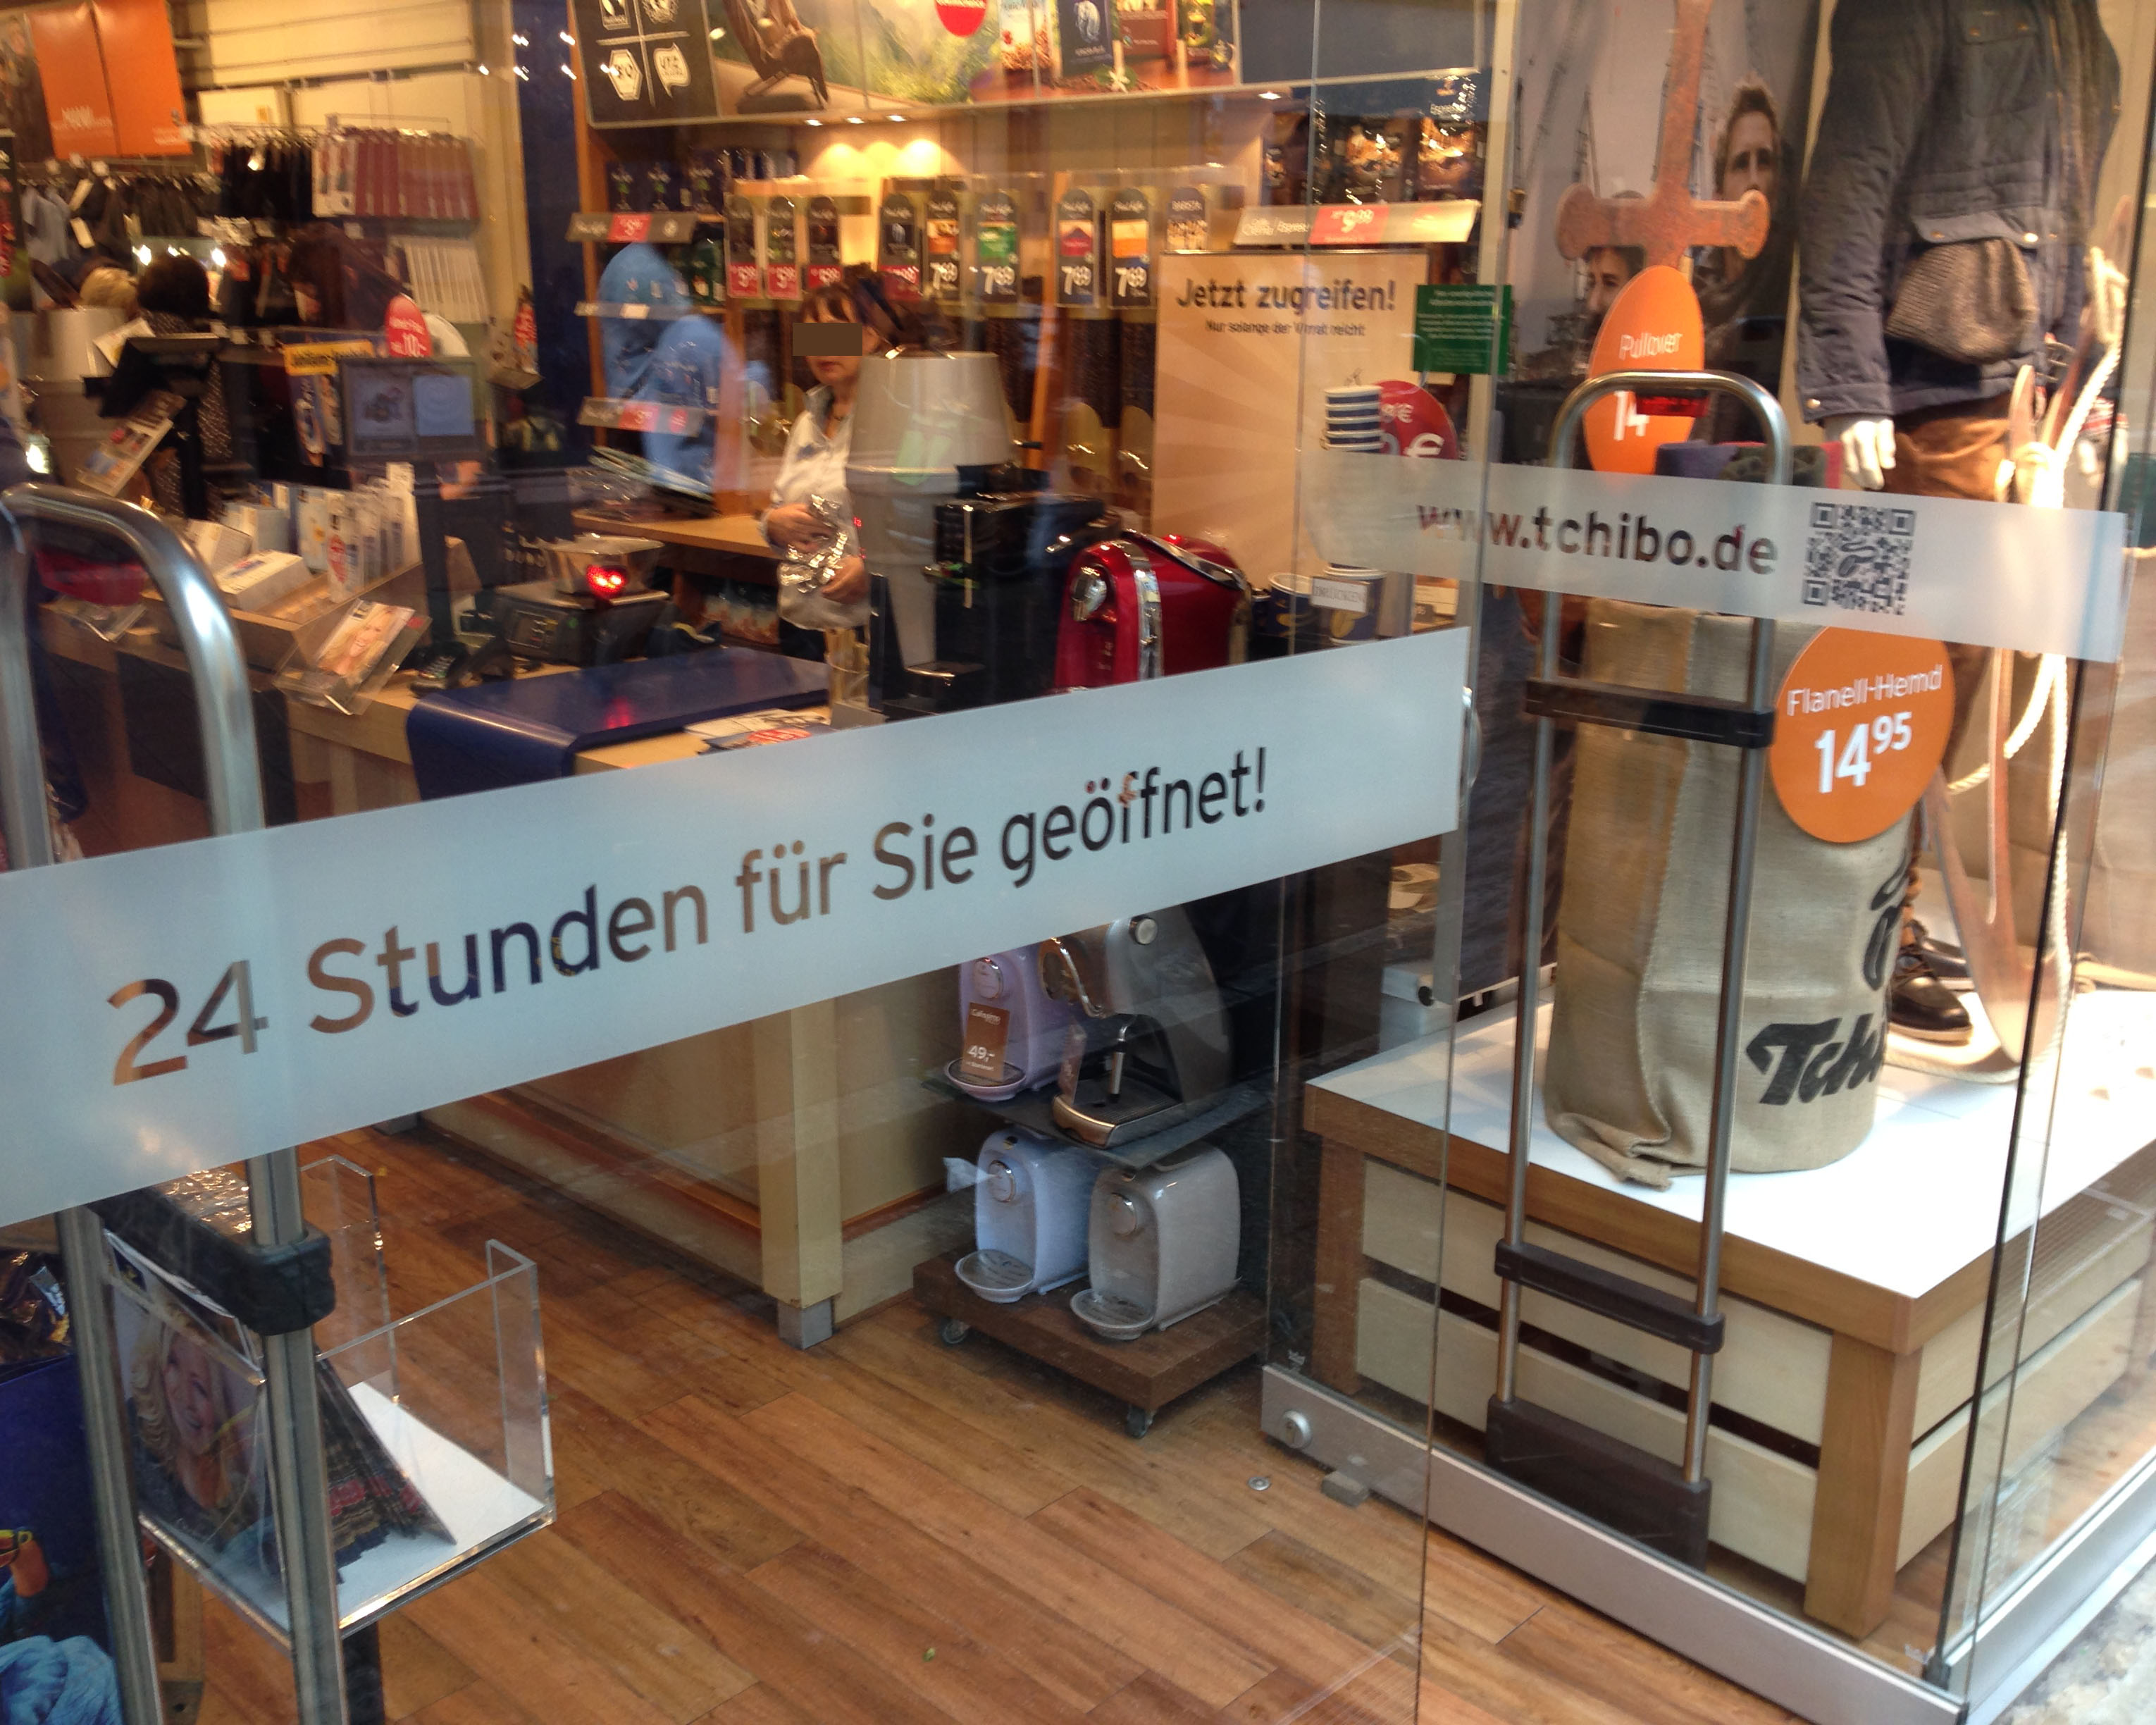
\includegraphics[width=0.4\textwidth]{Tschibo-24-7.jpg}
\caption{Angabe der URL bei Tschibo}
\label{pic:tschibourl}
\end{center}
\end{figure}

\subsubsection{Angabe von produktspezifischen Informationsseiten}

Problematischer wird es, wenn Links zu spezifischen Produktseiten in Webshop abgedruckt werden sollen. Die hier entstehenden \ac{URL}s sind i.d.R. eher lang und somit umständlich für den Kunden:\\ \url{http://www.manufactum.de/rollcontainer-stahlblech-p1470229/?a=66400}

Daher empfiehlt sich der Einsatz von sogenannten Kurz--URLs. Hier wird eine neue, deutlich kürzere \ac{URL} erzeugt, die den Besucher beim Aufruf auf die ursprüngliche Adresse umleitet. Technisch wird dies dadurch erreicht, dass der Hashwert einer langen Adresse an den Domainnamen des URL--Shorteners gehängt wird. Dadurch können viele lange Adressen auf jeweils
entsprechende Kurzlinks abgebildet werden: \url{http://goo.gl/QCJH55}\\
Dienste wie Ow.ly, Bit.ly, Goo.gl oder FixURL.de bieten entsprechende Dienste an, die per \ac{API} auch automatisiert genutzt werden können\footnote{siehe z.B. \url{http://dev.bitly.com/}}. Meist stellen diese Anbieter auch zumindest Aufrufstatistiken\footnote{z.B. Goo.gl} bis hin zu kompletten Analysedaten\footnote{z.B. Ow.ly durch das Social Media Management Tool Hootsuite} zur Vwerfügung.

Da der Kunde einer durch einen Dienst gekürzten \ac{URL} nicht mehr ansieht, wohin sie eigentlich führt, kann man durch die Verwendung eines eigenen, der Marke eindeutig zuordenbaren und dennoch kurzen Domainnamen verwenden. Hierdurch steigt das Vertrauen der Kunden in die Seriosität der aufgerufenen Webseite. Auch hat man die Kontrolle über die erzeugten Links und Statistiken.\footnote{vgl. \cite{webmag} sowie \cite{gillen}}

Kurz––URLs sind in Geschäften nicht weit verbreitet. Allerdings werden normale Internetadressen oft in Schaufenstern oder auf sonstigen Drucksachen beworben.\footnote{Eigene Beobachtung in den Innenstädten von Freiburg, Stuttgart und Frankfurt}

\subsection{Maschinenlesbare Internetadressen}

Ein \ac{QR--Code} ist eine weit verbreitete\footnote{vgl. \cite{statista:qr}} Form von 2D--Barcodes mit standardisierter Erzeugungsvorschrift\footnote{vgl. \cite{iso:qr} bzw. \url{http://www.qrcode.com/en/about/standards.html}}. Es besteht eine hinreichend große Auswahl an Diensten oder Programmen, die QR--Codes generieren und lesen können. Bei den Leseprogrammen ist besonders die Verbreitung der entsprechenden Smartphone--Apps interessant, dann durch diese erhalten Kunden mit Smartphone die Möglichkeit, \ac{URL}s direkt aus dem Katalog oder vom Preisschild im Ladengeschäft zu scannen und aufzurufen. 

Durch Platzierung von QR--Codes an den einzelnen Artikeln können Kunden direkt zu entsprechenden Web--Seiten im Online--Shop geleitet werden, um dort Zusatzinformationen oder Bewertungen anderer Kunden abzurufen. 

QR--Codes sind für viele Kunden als Link zu weiteren Informationen\footnote{wie z.B. bei den Artikeln mit erhöhtem Informationsbedarf in Abbildung \ref{pic:lidlqr}} direkt erkennbar. Eine Erklärung ist somit i.d.R. nicht notwendig, kann jedoch mit einem entsprechend plazierten menschenlesbaren Link implizit beigefügt werden. Eine entsprechende Gestaltung wie z.B. in Abbildung \ref{pic:aldiqr} kann eine herkömmliche Gebrauchsanweisung ebenfalls ersetzen.
\\Während die Erzeugung einzelner weniger QR--Codes individuell vorgenommen werden kann, ist bei einer Ausstattung von vielen oder allen Artikeln eine automatische Erzeugung per \ac{API} oder direkt im Shopsystem notwendig.

\begin{minipage}[t]{0.4\textwidth}
\begin{figure}[H]
\begin{center}
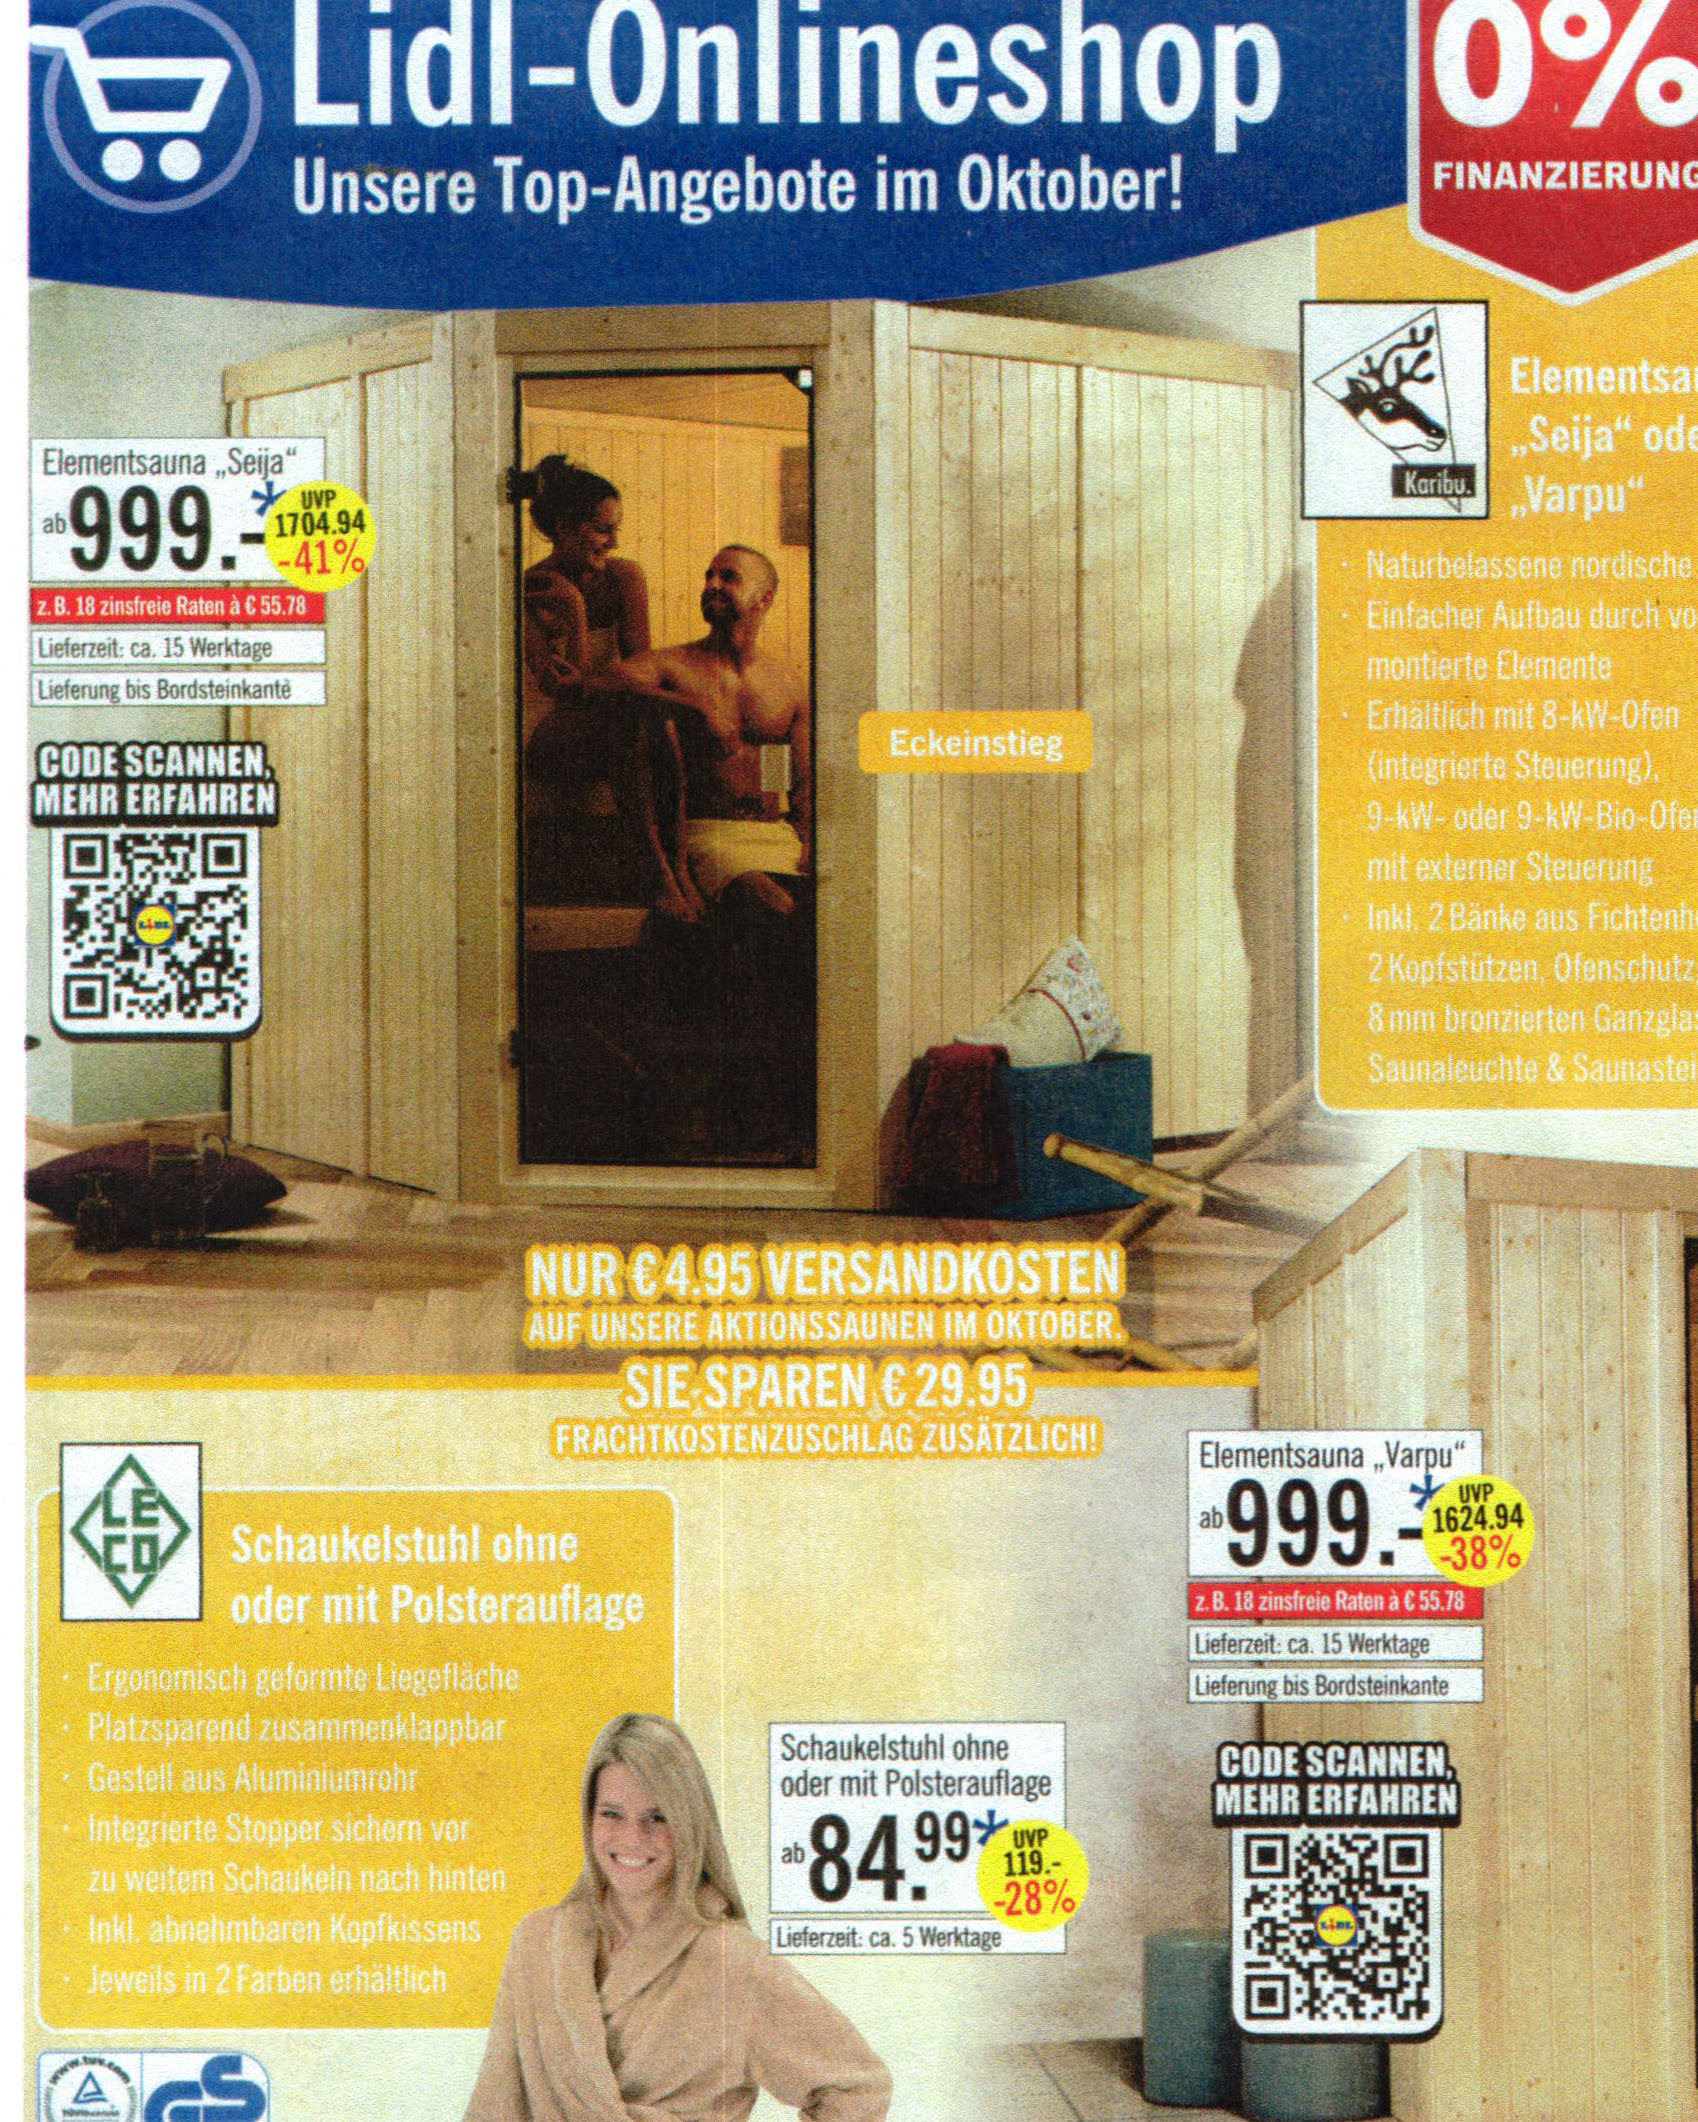
\includegraphics[width=\textwidth]{LIDL-QR.jpg}
\caption{Hinweis im Prospekt auf weitere Informationen bei LIDL}
\label{pic:lidlqr}
\end{center}
\end{figure}
\end{minipage}
\hfill
\begin{minipage}[t]{0.4\textwidth}
\begin{figure}[H]
\begin{center}
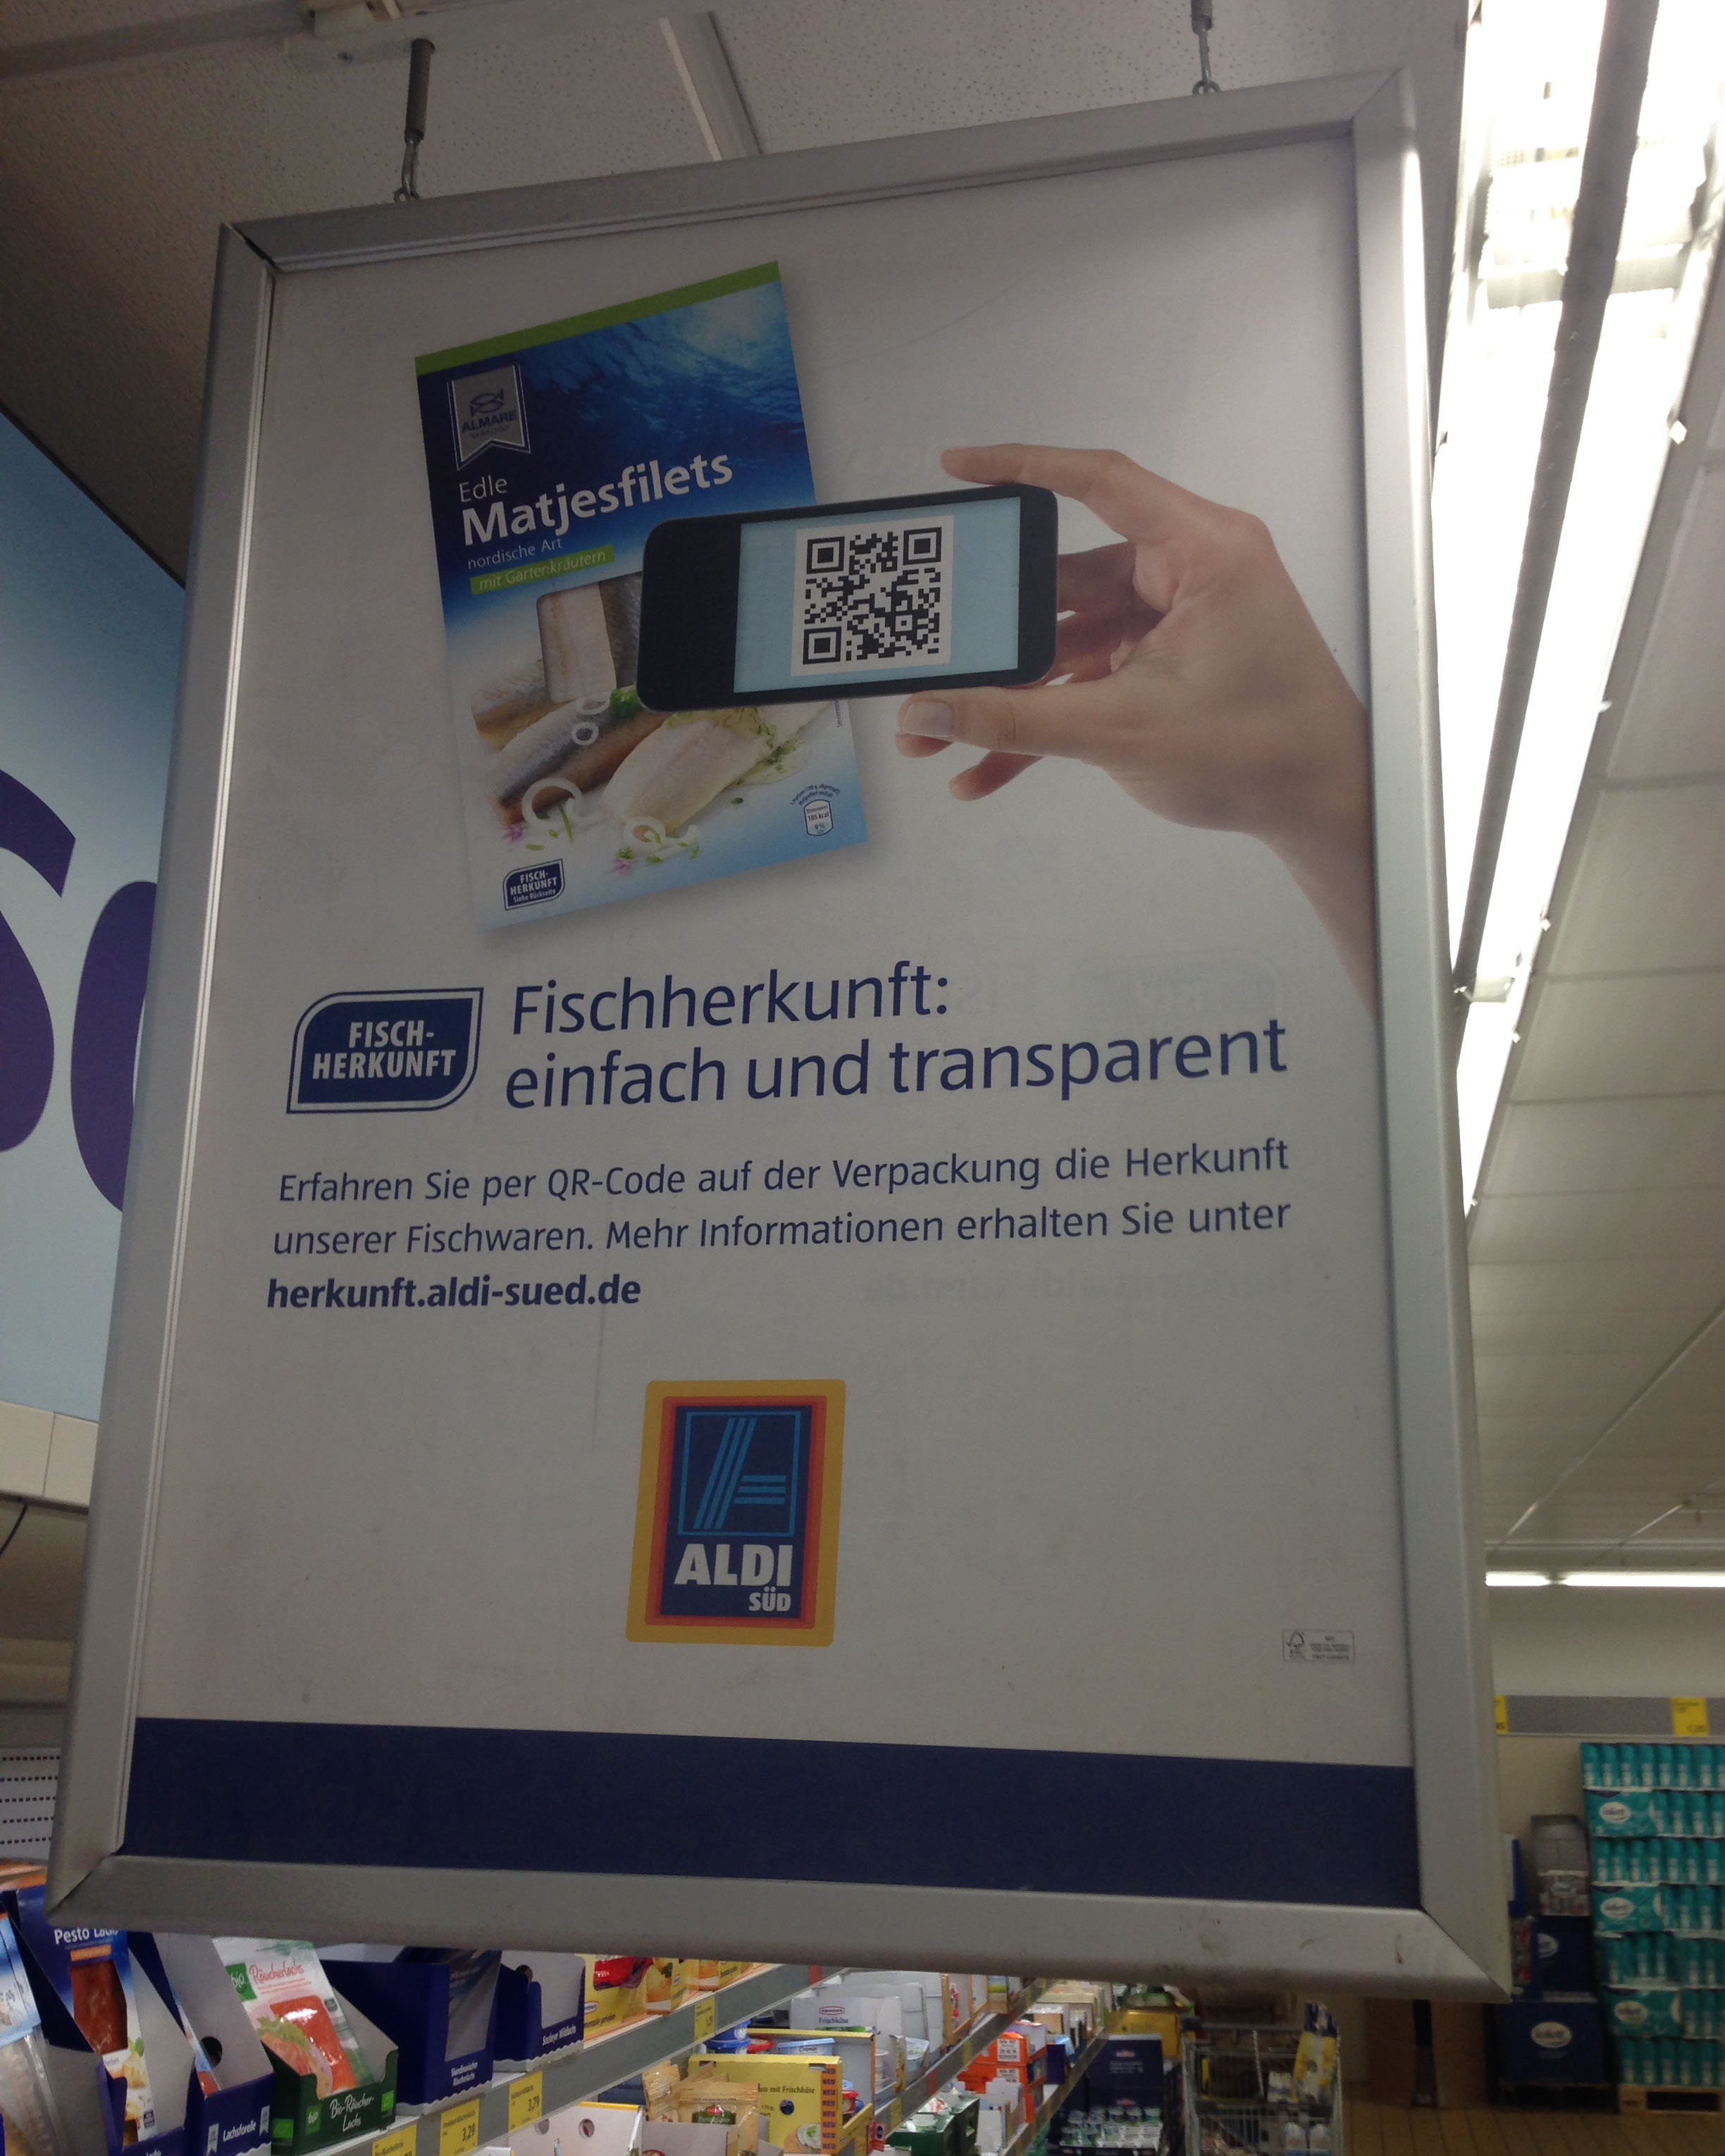
\includegraphics[width=\textwidth]{ALDI-QR.jpg}
\caption{Hinweis auf weitere Informationen bei ALDI--Süd}
\label{pic:aldiqr}
\end{center}
\end{figure}
\end{minipage}

\subsection{Verfügbarkeitsanzeige bzw. Bestellung zur Ansicht}
\label{bza}

In Webshops\footnote{z.B. Amazon.de, Alternate.de, aber auch bei Manufactum.de} wird oft basierend auf dem Lagerstand die erwartete Lieferzeit angegeben. Diese Funktionalität kann in sofern erweitert werden, dass die Verfügbarkeit in den Filialen angezeigt werden kann. Besucher des Webshops können somit erkennen, ob der Artikel vor Ort betrachtet bzw. direkt abgeholt oder zurückgegeben werden kann\footnote{Entsprechende Funktionalität ist z.B. bei Karstadt (siehe Abbildung \ref{pic:karstadtab}) und Deichmann (siehe Abbildung \ref{pic:deichmannab}), aber auch im Webshop von MediaMarkt (Artikel in Filiale … direkt erhältlich.) bzw. Obi (Reservieren und abholen) implementiert}. 

\begin{minipage}[t]{0.4\textwidth}
\begin{figure}[H]
\begin{center}
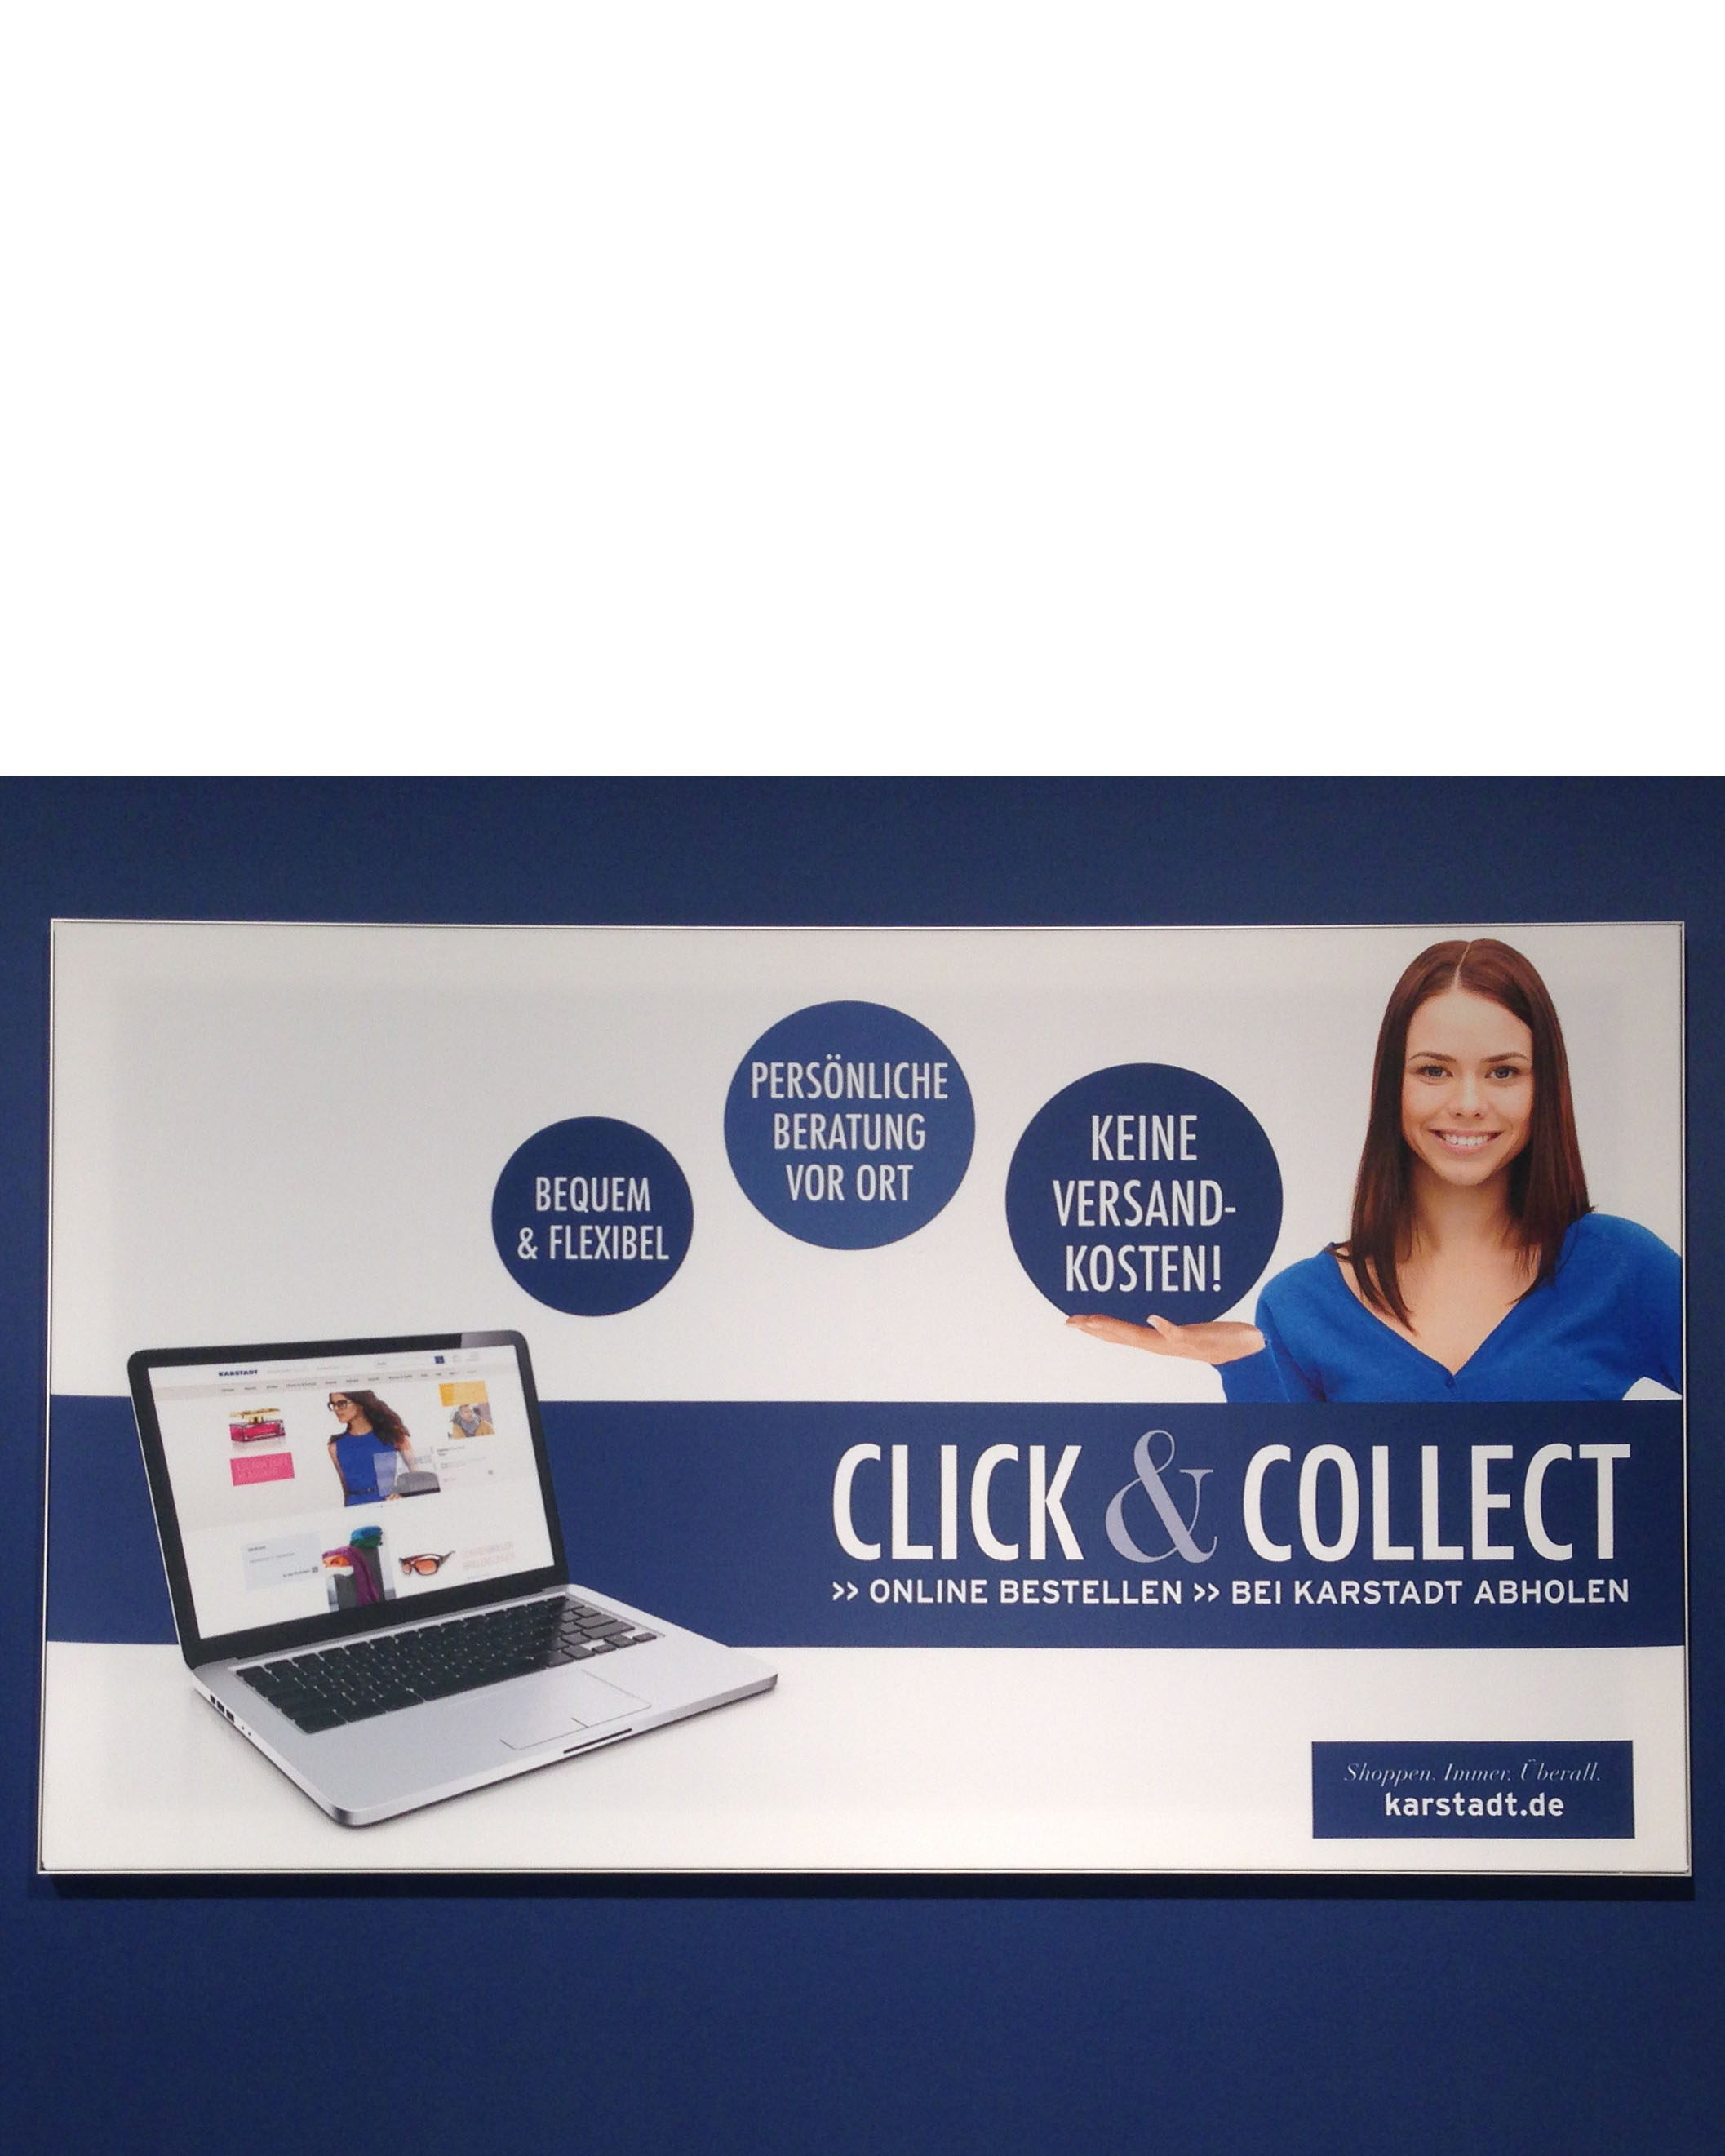
\includegraphics[width=\textwidth]{Karstadt-Abholung.jpg}
\caption{Bestellung in die Filiale bei Karstadt}
\label{pic:karstadtab}
\end{center}
\end{figure}
\end{minipage}
\hfill
\begin{minipage}[t]{0.4\textwidth}
\begin{figure}[H]
\begin{center}
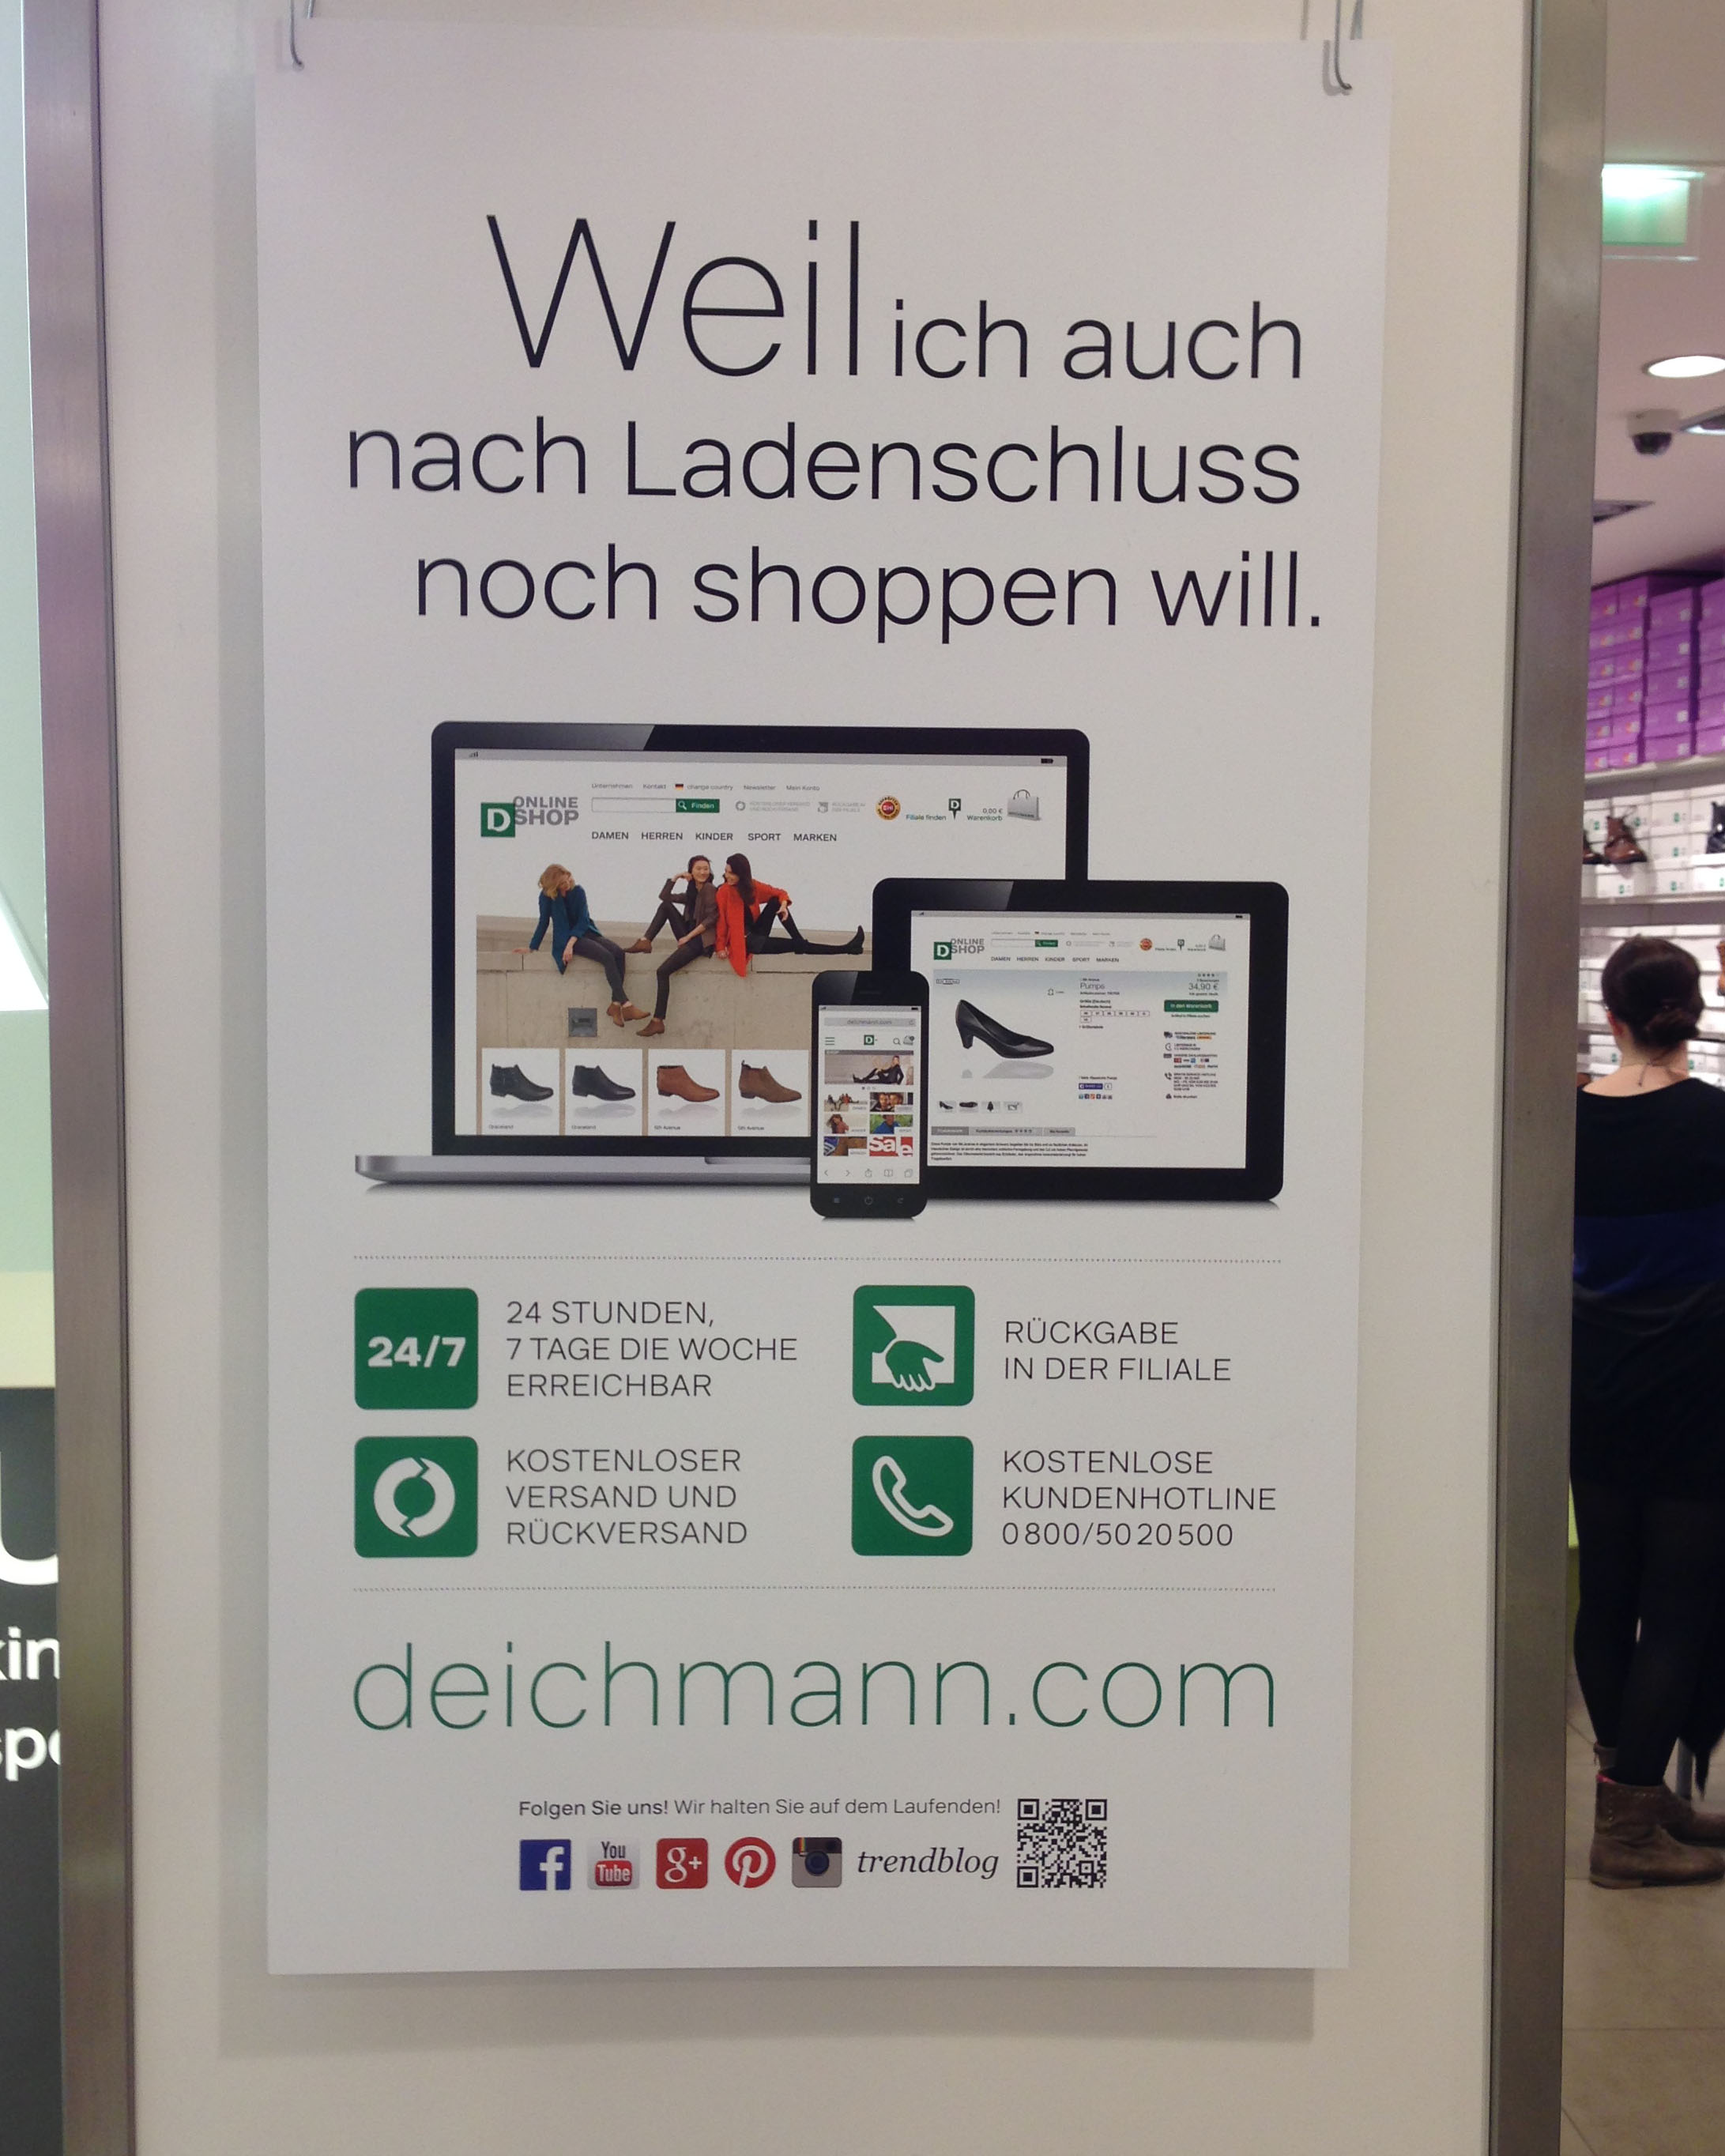
\includegraphics[width=\textwidth]{Deichmann-Rueckgabe.jpg}
\caption{Rückgabe von Online--Käufen in der Filiale bei Deichmann}
\label{pic:deichmannab}
\end{center}
\end{figure}
\end{minipage}

Hierdurch werden neben der Verknüpfung der beiden Verkaufskanäle weitere Effekte erzielt: Durch eine Reservierung auf der Website sinkt das Risiko, dass sich der Kunde für einen anderen Anbieter oder gegen einen Kauf entscheidet. Auch vermindert sich die Zahl der Rücksendungen, wenn der Kunde nicht „zur Ansicht“ nach Hause bestellt, sondern die Waren im Geschäft begutachten kann. Bei entsprechender Gestaltung der Texte und Konditionen wäre es evt. sogar möglich, den Kauf nicht mehr nach dem Fernabsatzgesetz sondern als regulärer Einkauf in der Filiale durchführen zu können. Des weiteren entfällt die Notwendigkeit, die Zahlung online abzuwickeln.

Um eine entsprechende Funktionalität im Webshop bieten zu können, ist es notwendig diesen eng in das \ac{ERP} zu integrieren. Es müssen die entsprechenden Lagerbestände von der Shopsoftware abgefragt werden können. Außerdem sind Vormerkungen bzw. Bestellungen zur Ansicht/Abholung an die entsprechenden Filialen weiterzuleiten.  Es werden also hohe Anforderungen an die Unternehmensprozesse sowie an die Echtzeitfähigkeit der Schnittstelle zwischen Webshop und ERP--System gestellt.

\subsection{Info--Terminal}

Kunden in einer Filiale können mit Hilfe eines Info–Terminals auf die Funktionen des Webshops zugreifen. Dadurch können momentan nicht im Geschäft vorrätige Artikel direkt bestellt und evt. vor Ort bezahlt werden. Hierdurch scheitert ein Kaufinteresse nicht an der begrenzten Lagerfähigkeit von Ladengeschäften.

Für die Ausgestaltung dieser Lösung stehen mehrere Möglichkeiten offen. Wie im klassischen Buchhandel ist es möglich, dass Verkaufsmitarbeiter an den Informationsterminals nach Artikeln suchen und diese zur Lieferung in die Filiale oder zum Kunden nach Hause bestellen. Auch denkbar sind Terminals auf PC–Basis, mit denen Kunden selbst im Web–Shop recherchieren und bestellen können\footnote{z.B. im Outlet des Versandhändlers Pearl in Auggen}. Am Markt sind aber auch spezielle Lösungen, die eine angepasste Version des Online–Shops auf einem Touch–Terminal präsentiert\footnote{z.B. Marks and Spencers, vgl. \cite{intelms}, aber auch Tschibo in Freiburg, vgl. Bild \ref{pic:tschiboit}}. Die Anpassung der Shop\-ober\-fläche an den Touchscreen kann hierbei manuell erfolgen, oder von einer entsprechenden Software automatisch vorgenommen werden\footnote{z.B. durch Nephele for polytouch, \url{www.polytouch.de}}.

Die Integration ins das \ac{ERP} erfolgt bei dieser Lösung durch die Nutzung des ohnehin schon vorhandenen Online–Shops. Allerdings sind hier entsprechende Liefer-- und Zahloptionen zu implementieren, damit die Waren auch wie in Abschnitt \myref{bza} beschrieben in die Filiale geliefert bzw. dort bezahlt werden können. 

\begin{figure}[H]
\begin{center}
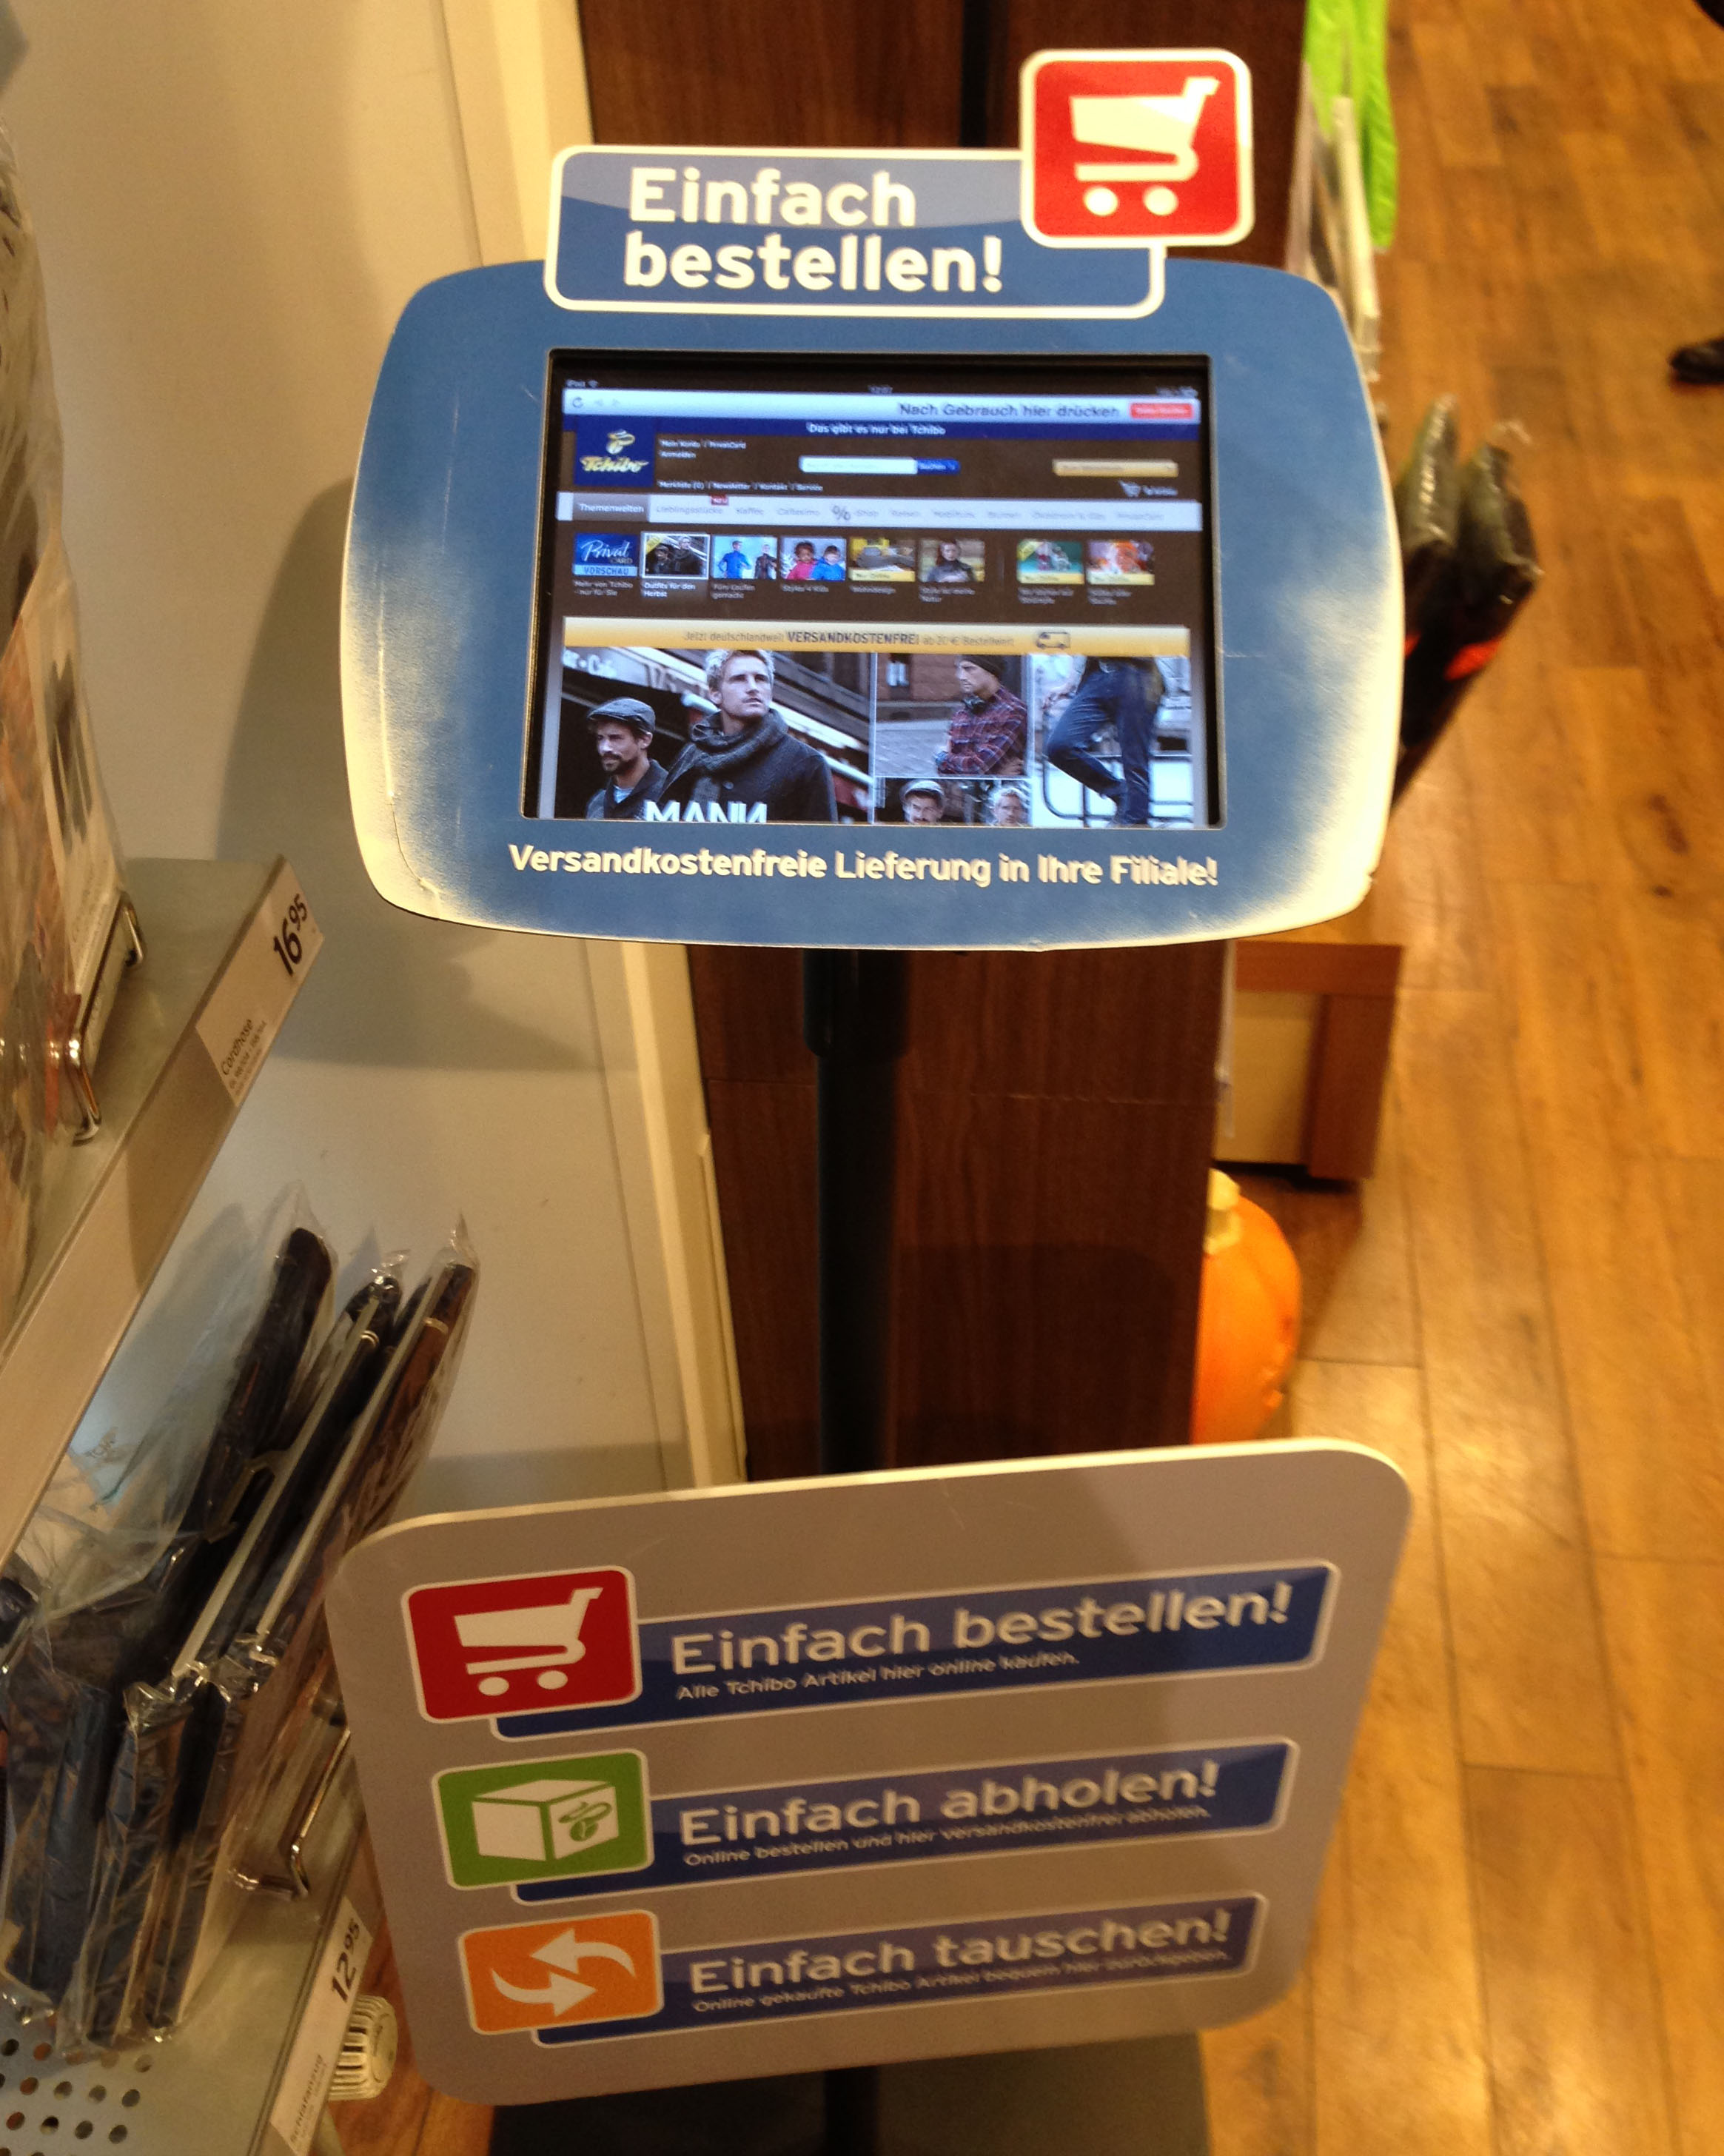
\includegraphics[width=0.4\textwidth]{Tschibo-Infoterminal.jpg}
\caption{Infoterminal bei Tschibo}
\label{pic:tschiboit}
\end{center}
\end{figure}

\section{Handlungsempfehlung}
\label{hempf}

Aufgrund der kostengünstigen Möglichkeiten der Herstellung von QR--Codes sowie den ausführlichen Informationen, die Manufactum über die angebotenen Artikel bereitstellt, empfiehlt sich die Angabe ebendieser, in Kombination mit menschenlesbaren Kurz--URLs. Um das Vertrauen der Kunden zu erhöhen sollten diese mit einen eigenen, dem Unternehmen zuordenbare Domainnamen erzeugt werden. Die maschinenlesbaren und menschenlesbaren URLs sollten unterscheidbar sein. Dadurch wird eine Auswertung bzgl. der genutzten Technik ermöglicht werden.

Ebenfalls empfehlenswert ist eine entsprechend aufbereitete Version des Web--Shops für Info--Terminals, die in den Filialen installiert werden. In der Einführungsphase können diese kostengünstig mit PC--Hardware realisiert werden.

Diese beiden Verknüpfungsarten eignen sich aufgrund der relativ geringen Laufzeiten gut für Lernphasen nach dem Trial and Error Prinzip. Mit jeder Neuauflage des Katalogs bzw. immer wenn Preisschilder gedruckt werden, kann man auf gemacht Erfahrungen zurückgreifen und Details den Erfordernissen anpassen.

Die Verfügbarkeitsanzeige bzw. die Bestellung der Waren in eine Filiale zur Ansicht scheint für Interessenten in der Nähe einer Filiale einen großen Kundennutzen zu erzeugen. Hier bestehen jedoch auch die höchsten Anforderungen an die zu Grunde liegende Software. Bei dieser Verknüpfungstechnik ist eine Anpassung der Prozessketten im Unternehmen notwendig, weshalb Änderungen deutlich länger dauern als bei den anderen Möglichkeiten. Eine Einführung erfordert somit bereits im Vorfeld eine gründliche Untersuchung und Planung. 

Da die in dieser Arbeit beschriebenen Techniken bereits etabliert und vielfach im Einsatz sind, ist eine rasche Umsetzung anzuraten.










